\documentclass[aspectratio=169,11pt]{beamer}

% =========================================================
% PACKAGES
% =========================================================
\usepackage[utf8]{inputenc}
\usepackage[T1]{fontenc}
\usepackage{lmodern}
\usepackage{amsmath,amssymb}
\usepackage{booktabs}
\usepackage{array}
\usepackage{tikz}
\usepackage{ragged2e}
\usepackage{graphicx}
\usepackage[table]{xcolor}
\usepackage{hyperref}

\usetikzlibrary{
    arrows.meta,
    positioning,
    shapes.geometric,
    shapes.misc,
    fit,
    calc
}

% =========================================================
% COLORS
% =========================================================
\definecolor{AmritaMaroon}{RGB}{165,0,55}
\definecolor{AmritaDark}{RGB}{95,0,35}
\definecolor{LightBlue}{RGB}{220,237,250}
\definecolor{LightGreen}{RGB}{224,244,228}
\definecolor{LightOrange}{RGB}{252,235,205}
\definecolor{LightPink}{RGB}{250,225,235}
\definecolor{LightGray}{RGB}{242,242,242}

% =========================================================
% THEME
% =========================================================
\usetheme{default}

\setbeamertemplate{navigation symbols}{}

\setbeamertemplate{frametitle}{
    \vspace{0.15cm}
    \begin{beamercolorbox}[
        wd=\paperwidth,
        ht=0.85cm,
        dp=0.15cm,
        leftskip=0.35cm
    ]{frametitle}
        \color{white}
        \Large\insertframetitle
    \end{beamercolorbox}
}

\setbeamercolor{frametitle}{bg=AmritaMaroon}
\setbeamercolor{normal text}{fg=black}
\setbeamercolor{structure}{fg=AmritaMaroon}

% =========================================================
% CUSTOM COMMANDS
% =========================================================

\newcommand{\subtitleline}[1]{
    \vspace{-0.05cm}
    {\small\color{AmritaDark}\textit{#1}}
    \vspace{0.15cm}
}

\newcommand{\highlight}[1]{
    \textbf{\color{AmritaMaroon}#1}
}

\newcommand{\bulletitem}[2]{
    \item \textbf{#1} #2
}

\newcommand{\infobox}[4]{
    \begin{tikzpicture}
        \node[
            rounded corners=5pt,
            fill=#1,
            inner sep=9pt,
            text width=#2
        ] {
            \textbf{\color{AmritaMaroon}#3}\\[3pt]
            #4
        };
    \end{tikzpicture}
}

% =========================================================
% TITLE
% =========================================================

\title{
    \textbf{Smart Home HAR for}\\
    \textbf{Speech-Impaired \& Hearing-Impaired Users}
}

\author{
    23CSE399 -- Project Phase 2\\[3mm]
    \small
    Adhikkesh S K \quad
    Adithya Ajay \quad
    Amrith B\\
    Gowreesh B \quad
    Rishiikesh S K
}

\institute{
    Department of Computer Science and Engineering\\
    Amrita Vishwa Vidyapeetham
}

\date{
    Guide Review 1 \;|\; Panel Review 1
}

% =========================================================
% DOCUMENT
% =========================================================

\begin{document}

% =========================================================
% TITLE SLIDE
% =========================================================

\begin{frame}
    \begin{tikzpicture}[remember picture,overlay]

        % Top label
        \node[
            anchor=north east,
            fill=AmritaMaroon,
            text=white,
            rounded corners=3pt,
            inner xsep=10pt,
            inner ysep=5pt
        ] at ([xshift=-0.25cm,yshift=-0.2cm]current page.north east)
        {\scriptsize Type 2: Application Project};

    \end{tikzpicture}

    \vspace{0.7cm}

    \begin{center}
        {\color{AmritaMaroon}\Large\bfseries
        Smart Home HAR for}\\[0.15cm]

        {\color{AmritaMaroon}\LARGE\bfseries
        Speech-Impaired \& Hearing-Impaired Users}

        \vspace{0.45cm}

        {\large 23CSE399 -- Project Phase 2}\\
        {\large Guide Review 1 \;|\; Panel Review 1}

        \vspace{0.45cm}

        \begin{tabular}{c}
        Adhikkesh S K\\
        Adithya Ajay\\
        Amrith B\\
        Gowreesh B\\
        Rishiikesh S K
        \end{tabular}

        \vspace{0.35cm}

        \textbf{Guide: Ms. Nalinadevi K}\\
        Department of CSE, Amrita Vishwa Vidyapeetham
    \end{center}
\end{frame}


% =========================================================
% 1. USE CASES
% =========================================================

\begin{frame}{1. Use Cases: Recognizing Activities in a Privacy-Preserving Smart Home}
\subtitleline{Two real-world situations motivating WiFi CSI based HAR}

\vspace{-0.1cm}
\begin{center}
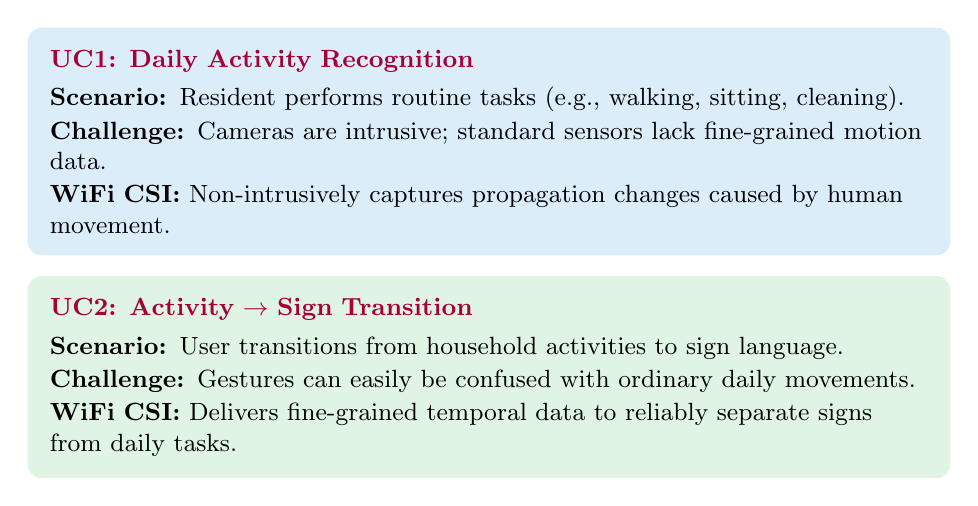
\begin{tikzpicture}[
    node distance=0.25cm,
    box/.style={
        rounded corners=5pt,
        inner sep=8pt,
        text width=0.92\textwidth,
        align=left,
        font=\small
    }
]

\node[box,fill=LightBlue] (uc1) {
    \textbf{\color{AmritaMaroon}UC1: Daily Activity Recognition}\\[3pt]
    \textbf{Scenario:} Resident performs routine tasks (e.g., walking, sitting, cleaning).\\[1pt]
    \textbf{Challenge:} Cameras are intrusive; standard sensors lack fine-grained motion data.\\[1pt]
    \textbf{WiFi CSI:} Non-intrusively captures propagation changes caused by human movement.
};

\node[box,fill=LightGreen,below=of uc1] (uc2) {
    \textbf{\color{AmritaMaroon}UC2: Activity $\rightarrow$ Sign Transition}\\[3pt]
    \textbf{Scenario:} User transitions from household activities to sign language.\\[1pt]
    \textbf{Challenge:} Gestures can easily be confused with ordinary daily movements.\\[1pt]
    \textbf{WiFi CSI:} Delivers fine-grained temporal data to reliably separate signs from daily tasks.
};

\end{tikzpicture}
\end{center}

\end{frame}


% =========================================================
% 2. USE CASE 3
% =========================================================

\begin{frame}{2. Use Cases: Multi-Channel CSI for Robust HAR}
\subtitleline{Extending CSI acquisition across non-overlapping WiFi channels}

\vspace{-0.1cm}
\begin{center}
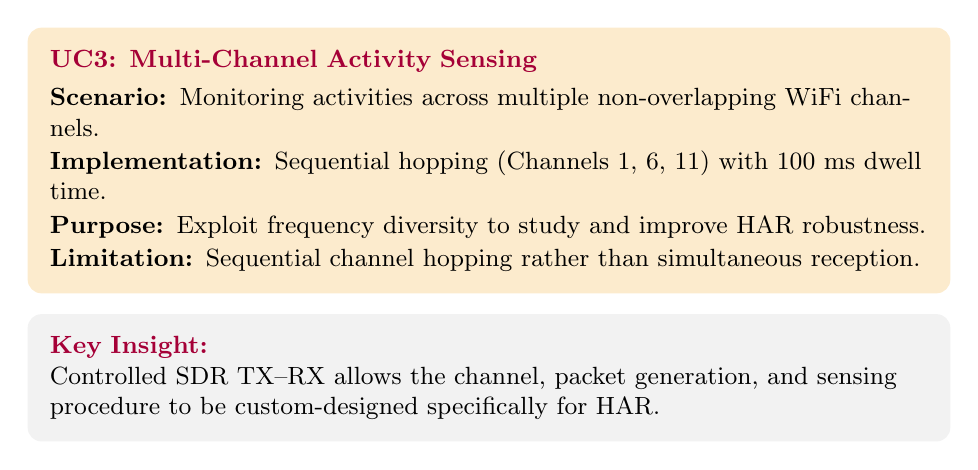
\begin{tikzpicture}[
    node distance=0.25cm,
    box/.style={
        rounded corners=5pt,
        inner sep=8pt,
        text width=0.92\textwidth,
        align=left,
        font=\small
    }
]

\node[box,fill=LightOrange] (uc3) {
    \textbf{\color{AmritaMaroon}UC3: Multi-Channel Activity Sensing}\\[3pt]
    \textbf{Scenario:} Monitoring activities across multiple non-overlapping WiFi channels.\\[1pt]
    \textbf{Implementation:} Sequential hopping (Channels 1, 6, 11) with 100 ms dwell time.\\[1pt]
    \textbf{Purpose:} Exploit frequency diversity to study and improve HAR robustness.\\[1pt]
    \textbf{Limitation:} Sequential channel hopping rather than simultaneous reception.
};

\node[
    rounded corners=5pt,
    fill=LightGray,
    inner sep=8pt,
    text width=0.92\textwidth,
    align=left,
    below=of uc3,
    font=\small
] (insight) {
    \textbf{\color{AmritaMaroon}Key Insight:}\\
    Controlled SDR TX--RX allows the channel, packet generation, and sensing procedure to be custom-designed specifically for HAR.
};

\end{tikzpicture}
\end{center}

\end{frame}


% =========================================================
% 3. MOTIVATION
% =========================================================

\begin{frame}{3. Motivation: Why Move to a Controlled SDR-Based CSI System?}

\vspace{0.15cm}

\begin{columns}[T,totalwidth=\textwidth]

% ---------------------------------------------------------
% LEFT COLUMN
% ---------------------------------------------------------

\column{0.48\textwidth}

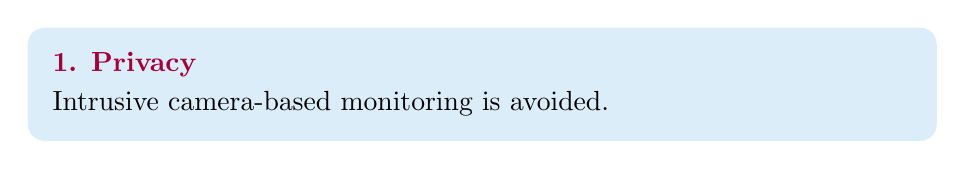
\begin{tikzpicture}
\node[
    rounded corners=6pt,
    fill=LightBlue,
    inner sep=9pt,
    text width=0.90\textwidth,
    align=left
] {
    \textbf{\color{AmritaMaroon}1. Privacy}\\[2pt]
    Intrusive camera-based monitoring is avoided.
};
\end{tikzpicture}

\vspace{0.16cm}

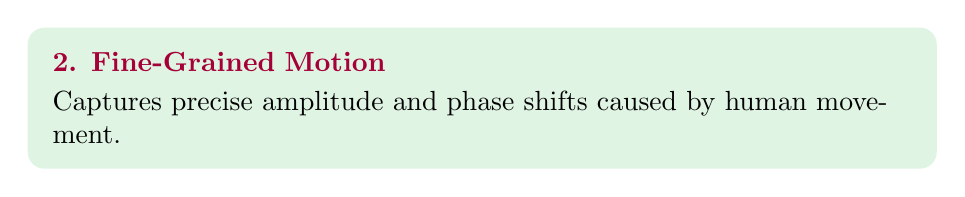
\begin{tikzpicture}
\node[
    rounded corners=6pt,
    fill=LightGreen,
    inner sep=9pt,
    text width=0.90\textwidth,
    align=left
] {
    \textbf{\color{AmritaMaroon}2. Fine-Grained Motion}\\[2pt]
    Captures precise amplitude and phase shifts caused by human movement.
};
\end{tikzpicture}

\vspace{0.16cm}

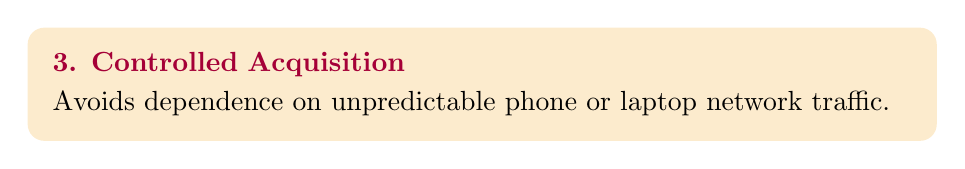
\begin{tikzpicture}
\node[
    rounded corners=6pt,
    fill=LightOrange,
    inner sep=9pt,
    text width=0.90\textwidth,
    align=left
] {
    \textbf{\color{AmritaMaroon}3. Controlled Acquisition}\\[2pt]
    Avoids dependence on unpredictable phone or laptop network traffic.
};
\end{tikzpicture}


% ---------------------------------------------------------
% RIGHT COLUMN
% ---------------------------------------------------------

\column{0.48\textwidth}

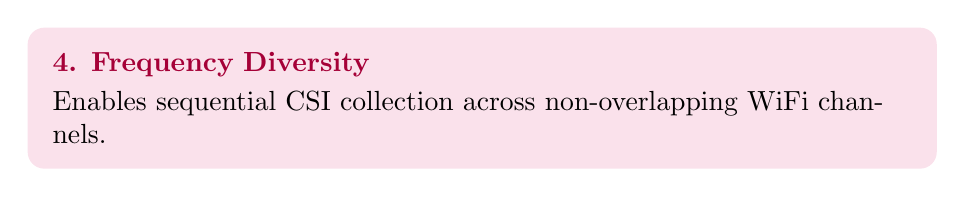
\begin{tikzpicture}
\node[
    rounded corners=6pt,
    fill=LightPink,
    inner sep=9pt,
    text width=0.90\textwidth,
    align=left
] {
    \textbf{\color{AmritaMaroon}4. Frequency Diversity}\\[2pt]
    Enables sequential CSI collection across non-overlapping WiFi channels.
};
\end{tikzpicture}

\vspace{0.16cm}

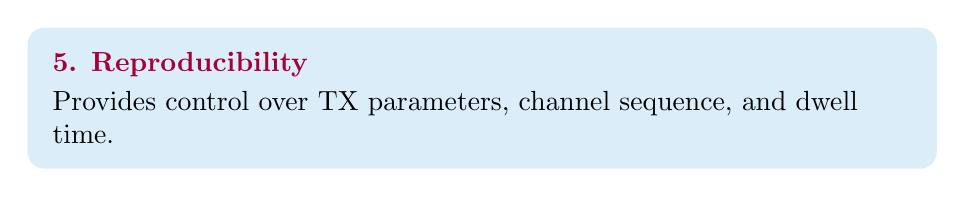
\begin{tikzpicture}
\node[
    rounded corners=6pt,
    fill=LightBlue,
    inner sep=9pt,
    text width=0.90\textwidth,
    align=left
] {
    \textbf{\color{AmritaMaroon}5. Reproducibility}\\[2pt]
    Provides control over TX parameters, channel sequence, and dwell time.
};
\end{tikzpicture}

\vspace{0.35cm}

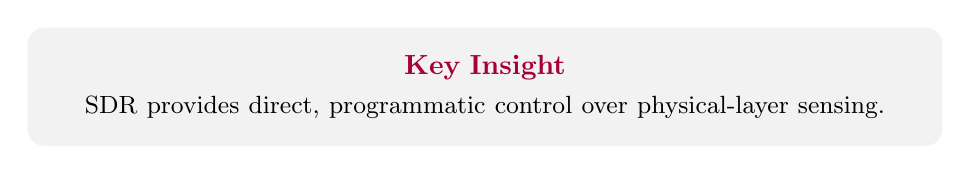
\begin{tikzpicture}
\node[
    rounded corners=6pt,
    fill=LightGray,
    inner sep=10pt,
    text width=0.90\textwidth,
    align=center
] {
    \textbf{\color{AmritaMaroon}Key Insight}\\[2pt]
    \small
    SDR provides direct, programmatic control over
    physical-layer sensing.
};
\end{tikzpicture}

\end{columns}

\end{frame}


% =========================================================
% 4. PROBLEM STATEMENT
% =========================================================

\begin{frame}{4. Problem Statement \& Research Objectives}
\subtitleline{Building a controlled, privacy-preserving CSI-HAR pipeline}

\vspace{-0.1cm}
\begin{center}
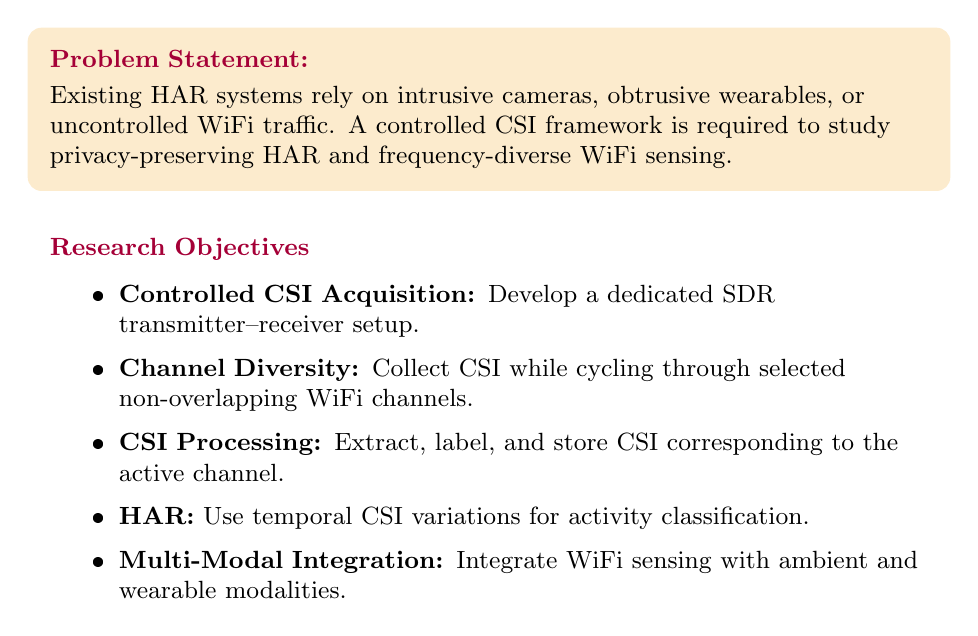
\begin{tikzpicture}[node distance=0.3cm]

\node[
    rounded corners=5pt,
    fill=LightOrange,
    inner sep=8pt,
    text width=0.92\textwidth,
    align=left,
    font=\small
] (prob) {
\textbf{\color{AmritaMaroon}Problem Statement:}\\[2pt]
Existing HAR systems rely on intrusive cameras, obtrusive wearables, or uncontrolled WiFi traffic. A controlled CSI framework is required to study privacy-preserving HAR and frequency-diverse WiFi sensing.
};

\node[
    below=of prob,
    text width=0.92\textwidth,
    align=left,
    font=\small
] (obj) {

\textbf{\color{AmritaMaroon}Research Objectives}

\begin{itemize}
    \setlength\itemsep{0.3em}
    \item \textbf{Controlled CSI Acquisition:} Develop a dedicated SDR transmitter--receiver setup.
    \item \textbf{Channel Diversity:} Collect CSI while cycling through selected non-overlapping WiFi channels.
    \item \textbf{CSI Processing:} Extract, label, and store CSI corresponding to the active channel.
    \item \textbf{HAR:} Use temporal CSI variations for activity classification.
    \item \textbf{Multi-Modal Integration:} Integrate WiFi sensing with ambient and wearable modalities.
\end{itemize}
};

\end{tikzpicture}
\end{center}

\end{frame}


% =========================================================
% 5. LITERATURE SURVEY
% =========================================================

\begin{frame}{5. Literature Survey}

\vspace{0.1cm}
\centering
\scriptsize
\renewcommand{\arraystretch}{1.25}
\setlength{\tabcolsep}{4pt}
\begin{tabular}{>{\bfseries\RaggedRight\arraybackslash}p{0.20\textwidth} >{\RaggedRight\arraybackslash}p{0.32\textwidth} >{\RaggedRight\arraybackslash}p{0.40\textwidth}}
\toprule
\rowcolor{AmritaMaroon}
{\color{white}Paper (Year)} & {\color{white}\textbf{Method / Technique}} & {\color{white}\textbf{Description}} \\
\midrule

\rowcolor{LightBlue}
SignFi \par (2018) &
9-layer CNN on WiFi CSI amplitude and phase &
Recognizes 276 sign-language gestures with 98\% lab accuracy; accuracy falls to 67\% for users unseen during training. \\
\midrule

\rowcolor{LightGreen}
Widar3.0 \par (2021) &
Domain-independent Body-coordinate Velocity Profile (BVP) + CNN--GRU &
Achieves zero-effort cross-domain gesture recognition (83--92\%), but requires line-of-sight and multiple synchronized WiFi links. \\
\midrule

\rowcolor{LightOrange}
ImgFi \par (2023) &
CSI converted to Recurrence-Plot images, classified by a lightweight 2D-CNN &
Reaches 99.5--99.8\% accuracy with $\sim$90$\times$ fewer parameters than ResNet50, but is evaluated within-domain only. \\
\midrule

\rowcolor{LightPink}
Joint Activity \& Localization \par (2019) &
Dual-branch 1D-CNN (ResNet1D) on CSI subcarrier fingerprints &
Jointly predicts activity (88\%) and indoor location (95.7\%) from CSI, but on a single-user, single-room dataset. \\
\bottomrule
\end{tabular}

\vspace{6pt}
\raggedright
{\color{AmritaMaroon}\scriptsize\bfseries Takeaway: }{\scriptsize Existing WiFi CSI systems are single-purpose (gesture-only or localization-only) and environment-specific. Our controlled multi-channel CSI pipeline aims to unify activity and sign-transition recognition in one privacy-preserving system.\par}

\end{frame}


% =========================================================
% 6. SYSTEM EVOLUTION + CURRENT ARCHITECTURE
% =========================================================

\begin{frame}{6. System Evolution: From Passive Capture to Controlled CSI}
\subtitleline{The major implementation change in the current phase}

\vspace{0.15cm}

\begin{columns}[T,totalwidth=\textwidth]

% ---------------- PREVIOUS ----------------

\column{0.45\textwidth}

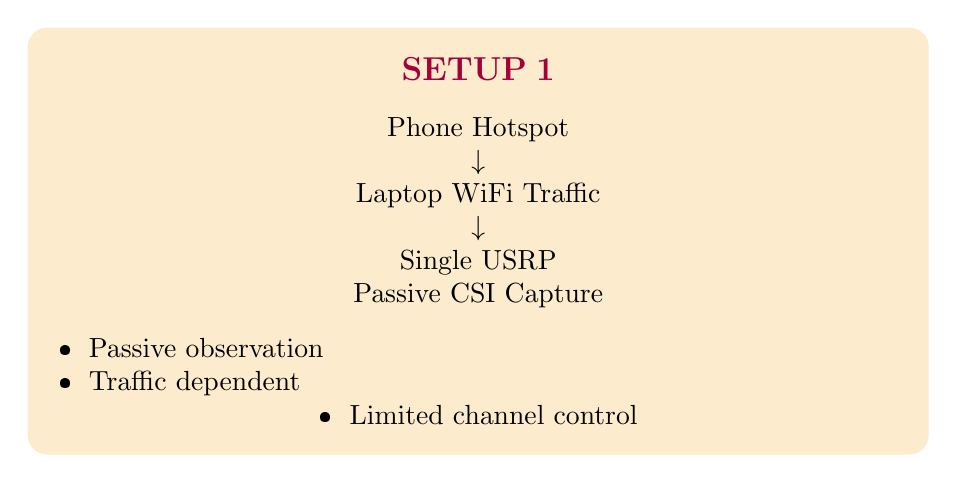
\begin{tikzpicture}
\node[
    rounded corners=7pt,
    fill=LightOrange,
    inner sep=11pt,
    text width=0.88\textwidth,
    align=center
] {
    {\large\bfseries\color{AmritaMaroon} SETUP 1}\\[8pt]

    Phone Hotspot\\
    $\downarrow$\\
    Laptop WiFi Traffic\\
    $\downarrow$\\
    Single USRP\\
    Passive CSI Capture\\[8pt]

    \raggedright
    \textbullet\; Passive observation\\
    \textbullet\; Traffic dependent\\
    \textbullet\; Limited channel control
};
\end{tikzpicture}

% ---------------- ARROW ----------------

\column{0.08\textwidth}

\begin{center}
\vspace{1.8cm}
{\Huge $\Rightarrow$}
\end{center}

% ---------------- CURRENT ----------------

\column{0.45\textwidth}

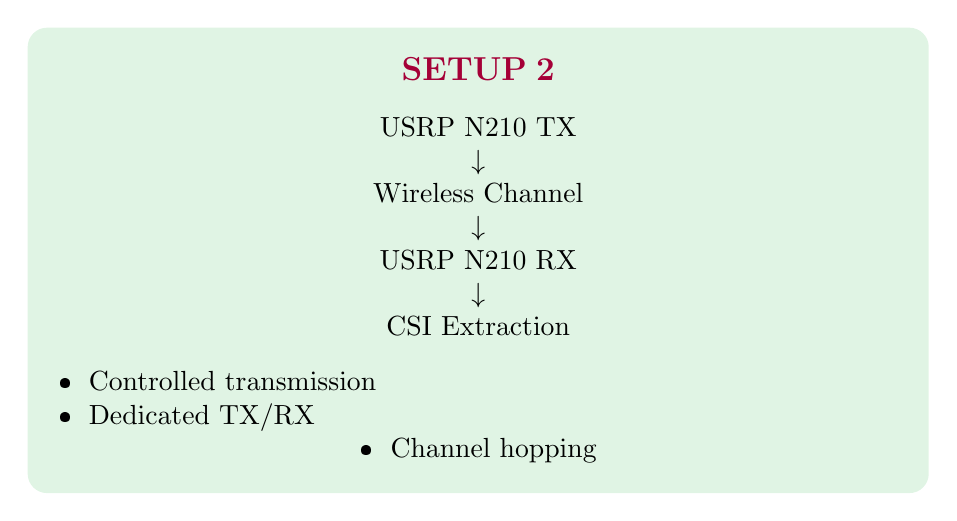
\begin{tikzpicture}
\node[
    rounded corners=7pt,
    fill=LightGreen,
    inner sep=11pt,
    text width=0.88\textwidth,
    align=center
] {
    {\large\bfseries\color{AmritaMaroon}SETUP 2}\\[8pt]

    USRP N210 TX\\
    $\downarrow$\\
    Wireless Channel\\
    $\downarrow$\\
    USRP N210 RX\\
    $\downarrow$\\
    CSI Extraction\\[8pt]

    \raggedright
    \textbullet\; Controlled transmission\\
    \textbullet\; Dedicated TX/RX\\
    \textbullet\; Channel hopping
};
\end{tikzpicture}

\end{columns}

\vspace{0.35cm}

\begin{center}
\textbf{\color{AmritaMaroon}Key change:}
From passive WiFi observation to a controlled SDR-based CSI platform.
\end{center}

\end{frame}


% =========================================================
% 7. CURRENT IMPLEMENTATION
% =========================================================

\begin{frame}{7. Current Implementation: Two-USRP CSI Setup}
\subtitleline{Controlled IEEE 802.11 transmission and sequential channel hopping}

\vspace{0.3cm}

\begin{center}

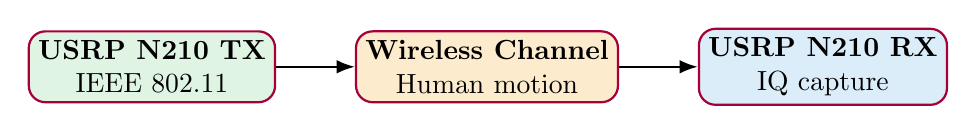
\begin{tikzpicture}[
    box/.style={
        rounded corners=6pt,
        minimum width=3.0cm,
        minimum height=0.9cm,
        align=center,
        draw=AmritaMaroon,
        thick
    },
    arr/.style={-{Latex},thick}
]

\node[box,fill=LightGreen] (tx)
{\textbf{USRP N210 TX}\\IEEE 802.11};

\node[box,fill=LightOrange,right=1.0cm of tx] (air)
{\textbf{Wireless Channel}\\Human motion};

\node[box,fill=LightBlue,right=1.0cm of air] (rx)
{\textbf{USRP N210 RX}\\IQ capture};

\draw[arr] (tx)--(air);
\draw[arr] (air)--(rx);

\end{tikzpicture}

\vspace{0.65cm}

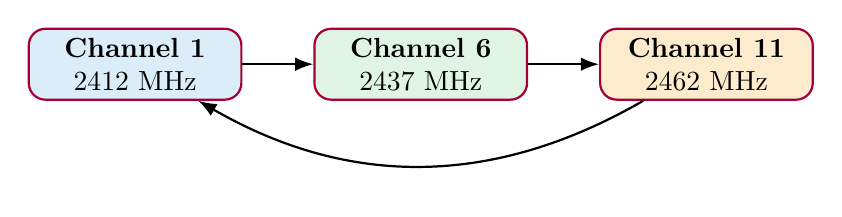
\begin{tikzpicture}[
    ch/.style={
        rounded corners=6pt,
        minimum width=2.7cm,
        minimum height=0.78cm,
        align=center,
        draw=AmritaMaroon,
        thick
    },
    arr/.style={-{Latex},thick}
]

\node[ch,fill=LightBlue] (c1)
{\textbf{Channel 1}\\2412 MHz};

\node[ch,fill=LightGreen,right=0.9cm of c1] (c6)
{\textbf{Channel 6}\\2437 MHz};

\node[ch,fill=LightOrange,right=0.9cm of c6] (c11)
{\textbf{Channel 11}\\2462 MHz};

\draw[arr] (c1)--(c6);
\draw[arr] (c6)--(c11);
\draw[arr] (c11) to[bend left=30] (c1);

\end{tikzpicture}

\vspace{0.5cm}

\begin{columns}[T,totalwidth=\textwidth]

\column{0.48\textwidth}

\begin{itemize}
    \item Controlled IEEE 802.11 transmission
    \item Dedicated SDR transmitter and receiver
\end{itemize}

\column{0.48\textwidth}

\begin{itemize}
    \item Sequential hopping across Channels 1, 6 and 11
    \item $\approx$100 ms dwell per channel
\end{itemize}

\end{columns}

\end{center}

\end{frame}

% =========================================================
% 8. CSI ACQUISITION PIPELINE
% =========================================================

\begin{frame}{8. CSI Acquisition Pipeline}
\subtitleline{Processing received 802.11 frames to extract CSI}

\vspace{0.25cm}

\begin{center}

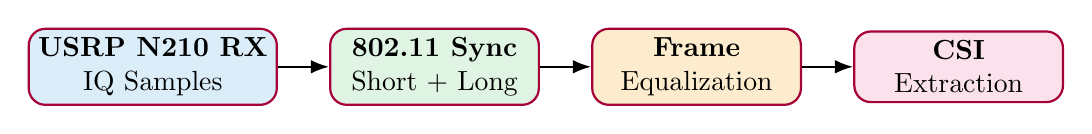
\begin{tikzpicture}[
    box/.style={
        rounded corners=6pt,
        minimum width=2.65cm,
        minimum height=0.82cm,
        align=center,
        draw=AmritaMaroon,
        thick
    },
    arr/.style={-{Latex},thick}
]

\node[box,fill=LightBlue] (iq)
{\textbf{USRP N210 RX}\\IQ Samples};

\node[box,fill=LightGreen,right=0.65cm of iq] (sync)
{\textbf{802.11 Sync}\\Short + Long};

\node[box,fill=LightOrange,right=0.65cm of sync] (eq)
{\textbf{Frame}\\Equalization};

\node[box,fill=LightPink,right=0.65cm of eq] (csi)
{\textbf{CSI}\\Extraction};

\draw[arr] (iq)--(sync);
\draw[arr] (sync)--(eq);
\draw[arr] (eq)--(csi);

\end{tikzpicture}

\vspace{0.55cm}

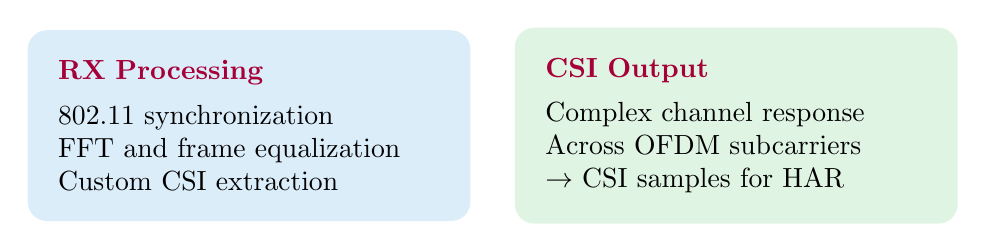
\begin{tikzpicture}[
    box/.style={
        rounded corners=7pt,
        inner sep=11pt,
        text width=0.40\textwidth,
        align=left
    }
]

\node[
    box,
    fill=LightBlue
] (processing) {
\textbf{\color{AmritaMaroon}RX Processing}\\[4pt]
802.11 synchronization\\
FFT and frame equalization\\
Custom CSI extraction
};

\node[
    box,
    fill=LightGreen,
    right=0.55cm of processing
] (output) {
\textbf{\color{AmritaMaroon}CSI Output}\\[4pt]
Complex channel response\\
Across OFDM subcarriers\\
$\rightarrow$ CSI samples for HAR
};

\end{tikzpicture}

\vspace{0.4cm}

\textbf{\color{AmritaMaroon}Key result:}
Received WiFi frames are converted into CSI measurements
for subsequent HAR analysis.

\end{center}

\end{frame}
% =========================================================
% 9. IMPORTANT DISTINCTION
% =========================================================

\begin{frame}{9. Current Capability vs. Future Extension}
\subtitleline{Clarifying what the present implementation achieves}

\begin{columns}[T]

% =========================================================
% CURRENT
% =========================================================

\column{0.47\textwidth}

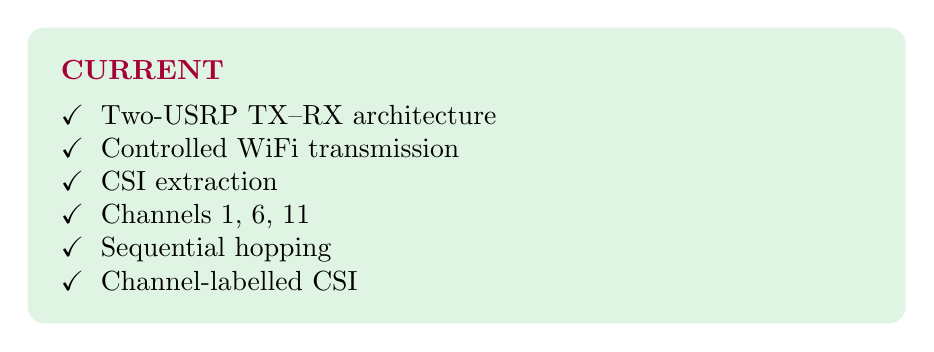
\begin{tikzpicture}
\node[
    rounded corners=6pt,
    fill=LightGreen,
    inner sep=12pt,
    text width=0.85\textwidth,
    align=left
] {
\textbf{\color{AmritaMaroon}CURRENT}\\[4pt]

\checkmark\; Two-USRP TX--RX architecture\\
\checkmark\; Controlled WiFi transmission\\
\checkmark\; CSI extraction\\
\checkmark\; Channels 1, 6, 11\\
\checkmark\; Sequential hopping\\
\checkmark\; Channel-labelled CSI
};
\end{tikzpicture}

% =========================================================
% FUTURE
% =========================================================

\column{0.47\textwidth}

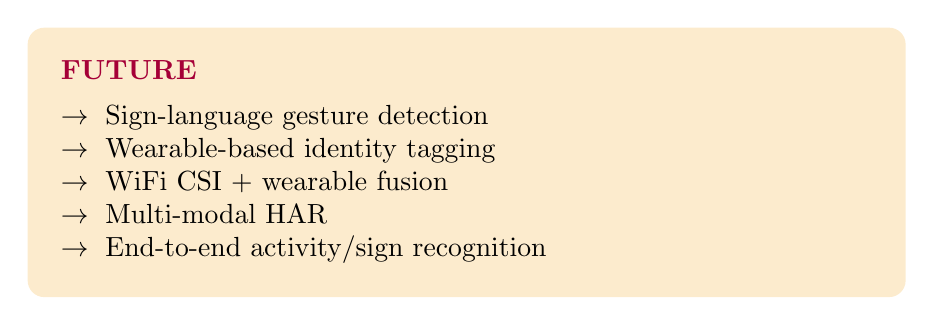
\begin{tikzpicture}
\node[
    rounded corners=6pt,
    fill=LightOrange,
    inner sep=12pt,
    text width=0.85\textwidth,
    align=left
] {
\textbf{\color{AmritaMaroon}FUTURE}\\[4pt]

$\rightarrow$\; Sign-language gesture detection\\
$\rightarrow$\; Wearable-based identity tagging\\
$\rightarrow$\; WiFi CSI + wearable fusion\\
$\rightarrow$\; Multi-modal HAR\\
$\rightarrow$\; End-to-end activity/sign recognition
};
\end{tikzpicture}

\end{columns}

\vspace{0.45cm}

\begin{center}
\textbf{Important:}
The present two-USRP system hops between channels; it does
\textbf{not} receive Channels 1, 6 and 11 simultaneously.
\end{center}

\end{frame}
% =========================================================
% 10. CSI DATA
% =========================================================

\begin{frame}{10. CSI Data: From Channel Response to HAR Input}
\subtitleline{What is extracted from each received WiFi frame}

\vspace{0.2cm}

\begin{center}

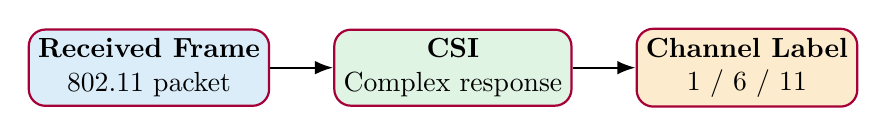
\begin{tikzpicture}[
    box/.style={
        rounded corners=6pt,
        minimum width=2.7cm,
        minimum height=0.78cm,
        align=center,
        draw=AmritaMaroon,
        thick
    },
    arr/.style={-{Latex},thick}
]

\node[box,fill=LightBlue] (frame)
{\textbf{Received Frame}\\802.11 packet};

\node[box,fill=LightGreen,right=0.8cm of frame] (csi)
{\textbf{CSI}\\Complex response};

\node[box,fill=LightOrange,right=0.8cm of csi] (label)
{\textbf{Channel Label}\\1 / 6 / 11};

\draw[arr] (frame)--(csi);
\draw[arr] (csi)--(label);

\end{tikzpicture}

\vspace{0.5cm}

\begin{columns}[T,totalwidth=\textwidth]

\column{0.48\textwidth}

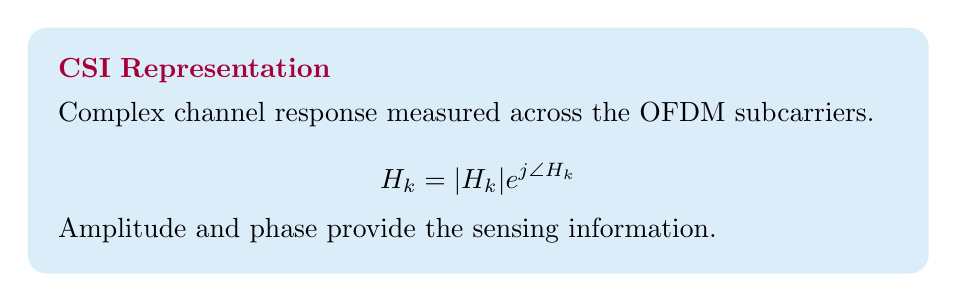
\begin{tikzpicture}
\node[
    rounded corners=7pt,
    fill=LightBlue,
    inner sep=11pt,
    text width=0.88\textwidth,
    align=left
] {
\textbf{\color{AmritaMaroon}CSI Representation}\\[4pt]

Complex channel response measured across
the OFDM subcarriers.

\[
H_k = |H_k|e^{j\angle H_k}
\]

Amplitude and phase provide the sensing information.
};
\end{tikzpicture}

\column{0.48\textwidth}

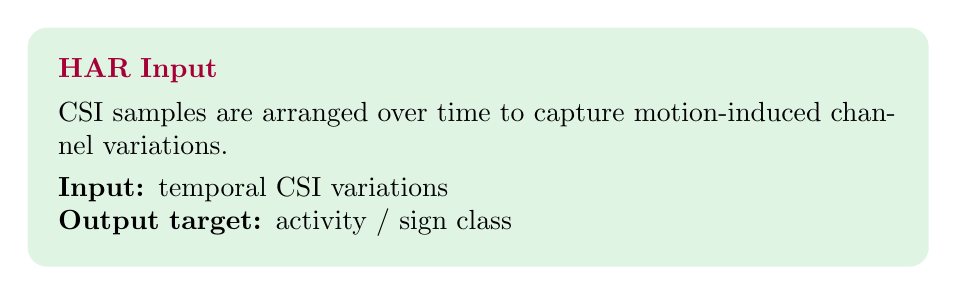
\begin{tikzpicture}
\node[
    rounded corners=7pt,
    fill=LightGreen,
    inner sep=11pt,
    text width=0.88\textwidth,
    align=left
] {
\textbf{\color{AmritaMaroon}HAR Input}\\[4pt]

CSI samples are arranged over time to capture
motion-induced channel variations.

\vspace{3pt}

\textbf{Input:} temporal CSI variations\\
\textbf{Output target:} activity / sign class
};
\end{tikzpicture}

\end{columns}

\vspace{0.35cm}

\textbf{\color{AmritaMaroon}Key result:}
Each CSI sample is associated with the active WiFi channel,
enabling channel-aware HAR analysis.

\end{center}

\end{frame}

% =========================================================
% 11. CSI PROCESSING AND SOFTWARE ARCHITECTURE
% =========================================================

\begin{frame}{11. CSI Processing and Software Architecture}
\subtitleline{GNU Radio + UHD + Python channel control + custom CSI extraction}

\vspace{0.1cm}

\begin{center}

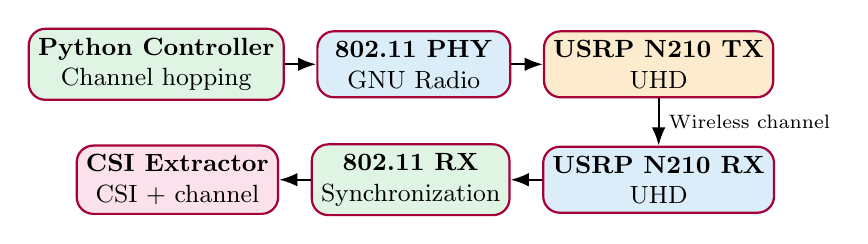
\begin{tikzpicture}[
    box/.style={
        rounded corners=6pt,
        minimum width=2.45cm,
        minimum height=0.6cm, % Reduced height slightly
        align=center,
        draw=AmritaMaroon,
        thick,
        font=\small % Added to reduce text size slightly
    },
    arr/.style={-{Latex},thick}
]

% =========================================================
% TX SIDE
% =========================================================

\node[
    box,
    fill=LightGreen
] (controller)
{\textbf{Python Controller}\\Channel hopping};

\node[
    box,
    fill=LightBlue,
    right=0.4cm of controller % Tightened gap
] (txphy)
{\textbf{802.11 PHY}\\GNU Radio};

\node[
    box,
    fill=LightOrange,
    right=0.4cm of txphy % Tightened gap
] (txusrp)
{\textbf{USRP N210 TX}\\UHD};

% =========================================================
% RX SIDE
% =========================================================

\node[
    box,
    fill=LightBlue,
    below=0.6cm of txusrp % Tightened vertical gap
] (rxusrp)
{\textbf{USRP N210 RX}\\UHD};

\node[
    box,
    fill=LightGreen,
    left=0.4cm of rxusrp % Tightened gap
] (sync)
{\textbf{802.11 RX}\\Synchronization};

\node[
    box,
    fill=LightPink,
    left=0.4cm of sync % Tightened gap
] (csi)
{\textbf{CSI Extractor}\\CSI + channel};

% =========================================================
% CONNECTIONS
% =========================================================

\draw[arr] (controller)--(txphy);
\draw[arr] (txphy)--(txusrp);

\draw[arr] (txusrp) -- node[right,font=\scriptsize]
{Wireless channel} (rxusrp);

\draw[arr] (rxusrp)--(sync);
\draw[arr] (sync)--(csi);

\end{tikzpicture}

\vspace{0.2cm} % Reduced vertical space

\begin{columns}[T,totalwidth=\textwidth]

\column{0.48\textwidth}

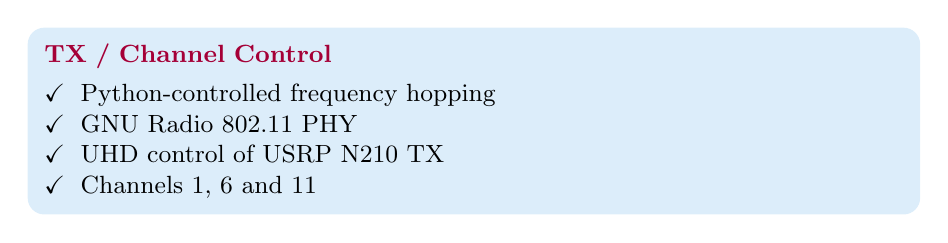
\begin{tikzpicture}
\node[
    rounded corners=6pt,
    fill=LightBlue,
    inner sep=6pt, % Reduced padding
    text width=0.9\textwidth,
    align=left,
    font=\small % Scaled down font to prevent word wrap overflow
] {
\textbf{\color{AmritaMaroon}TX / Channel Control}\\[3pt]
$\checkmark$\; Python-controlled frequency hopping\\
$\checkmark$\; GNU Radio 802.11 PHY\\
$\checkmark$\; UHD control of USRP N210 TX\\
$\checkmark$\; Channels 1, 6 and 11
};
\end{tikzpicture}

\column{0.48\textwidth}

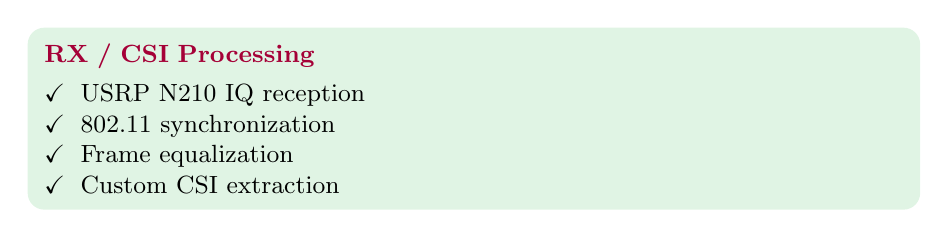
\begin{tikzpicture}
\node[
    rounded corners=6pt,
    fill=LightGreen,
    inner sep=6pt, % Reduced padding
    text width=0.9\textwidth,
    align=left,
    font=\small % Scaled down font
] {
\textbf{\color{AmritaMaroon}RX / CSI Processing}\\[3pt]
$\checkmark$\; USRP N210 IQ reception\\
$\checkmark$\; 802.11 synchronization\\
$\checkmark$\; Frame equalization\\
$\checkmark$\; Custom CSI extraction
};
\end{tikzpicture}

\end{columns}

\vspace{0.15cm} % Reduced vertical space

{\small \textbf{\color{AmritaMaroon}Current output:}
CSI measurements associated with the active channel.}

\end{center}

\end{frame}
% =========================================================
% 12. ACTIVE VS PASSIVE CSI SENSING
% =========================================================

\begin{frame}{12. Active vs. Passive CSI Sensing}
\subtitleline{Two paradigms for acquiring WiFi Channel State Information}

\vspace{-0.05cm}

\begin{columns}[T,totalwidth=\textwidth]

% =========================================================
% PASSIVE SENSING
% =========================================================

\column{0.48\textwidth}

\begin{center}
{\bfseries\color{AmritaMaroon} Passive Sensing}
\end{center}

\vspace{0.08cm}

\begin{center}
\begin{minipage}[c][2.7cm][c]{0.95\linewidth}
\centering
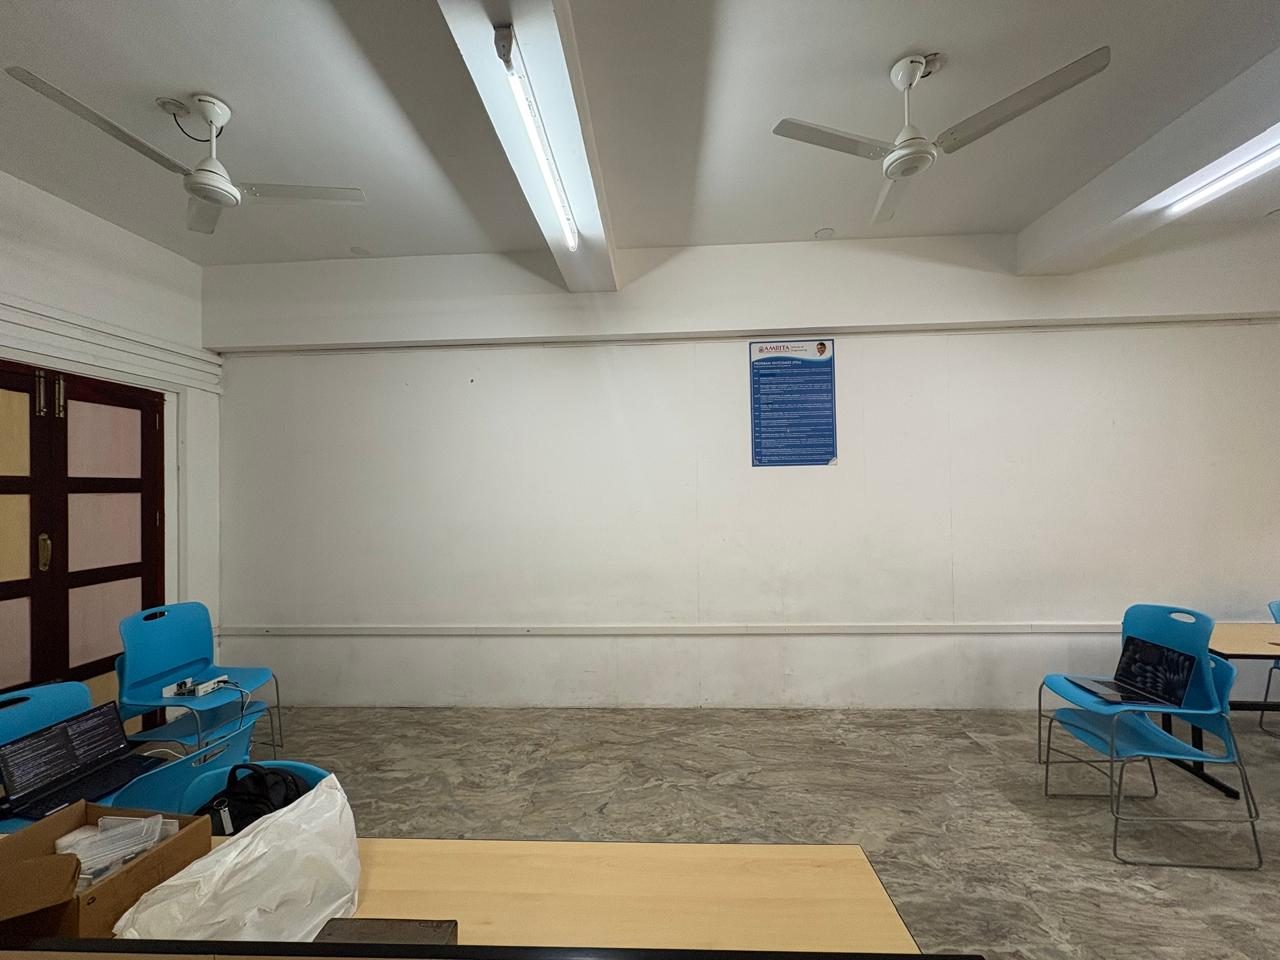
\includegraphics[width=\linewidth,height=2.7cm,keepaspectratio]{Passive.jpeg}
\end{minipage}
\end{center}

\vspace{0.12cm}

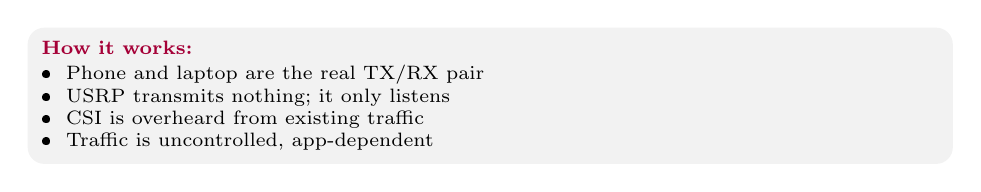
\begin{tikzpicture}
\node[
    rounded corners=6pt,
    fill=LightGray,
    inner sep=5pt,
    text width=0.94\textwidth,
    align=left,
    font=\scriptsize
] {
\textbf{\color{AmritaMaroon}How it works:}\\[1pt]
\raggedright
\textbullet\; Phone and laptop are the real TX/RX pair\\
\textbullet\; USRP transmits nothing; it only listens\\
\textbullet\; CSI is overheard from existing traffic\\
\textbullet\; Traffic is uncontrolled, app-dependent
};
\end{tikzpicture}

% =========================================================
% ACTIVE SENSING
% =========================================================

\column{0.48\textwidth}

\begin{center}
{\bfseries\color{AmritaMaroon} Active Sensing}
\end{center}

\vspace{0.08cm}

\begin{center}
\begin{minipage}[c][2.7cm][c]{0.95\linewidth}
\centering
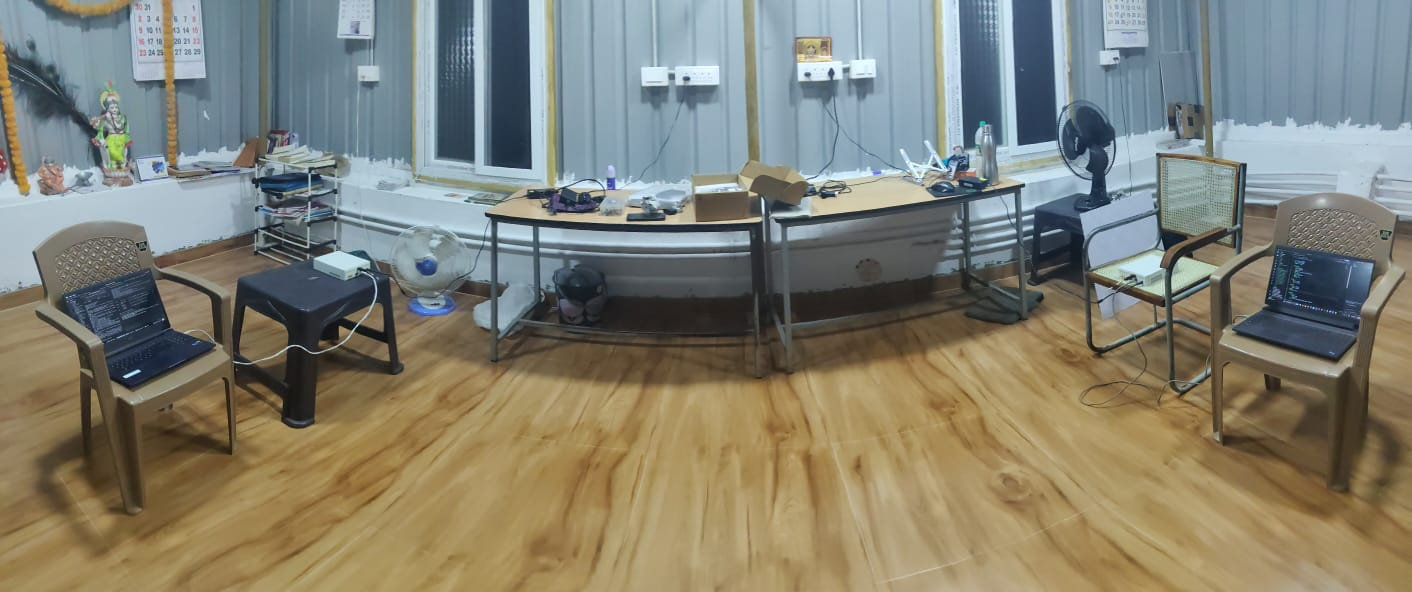
\includegraphics[width=\linewidth,height=2.7cm,keepaspectratio]{Active.jpeg}
\end{minipage}
\end{center}

\vspace{0.12cm}

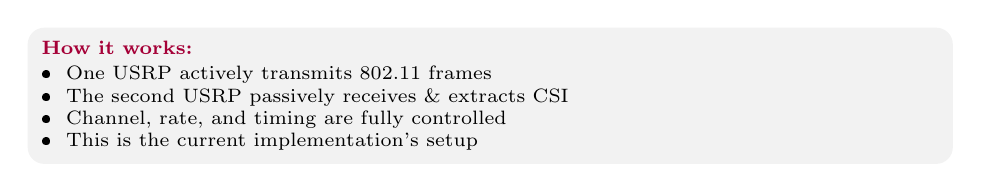
\begin{tikzpicture}
\node[
    rounded corners=6pt,
    fill=LightGray,
    inner sep=5pt,
    text width=0.94\textwidth,
    align=left,
    font=\scriptsize
] {
\textbf{\color{AmritaMaroon}How it works:}\\[1pt]
\raggedright
\textbullet\; One USRP actively transmits 802.11 frames\\
\textbullet\; The second USRP passively receives \& extracts CSI\\
\textbullet\; Channel, rate, and timing are fully controlled\\
\textbullet\; This is the current implementation's setup
};
\end{tikzpicture}

\end{columns}

\vspace{0.15cm}

\begin{center}
\small
\textbf{\color{AmritaMaroon}Key Insight:}
Passive sensing eavesdrops on someone else's traffic; active sensing uses a dedicated TX--RX pair for reliable, repeatable CSI.
\end{center}

\end{frame}


% =========================================================
% 13. LIMITATIONS + FUTURE WORK
% =========================================================

\begin{frame}{13. Limitations and Future Work}
\subtitleline{What remains before full sign-language recognition}

\begin{columns}[T,totalwidth=\textwidth]

\column{0.48\textwidth}

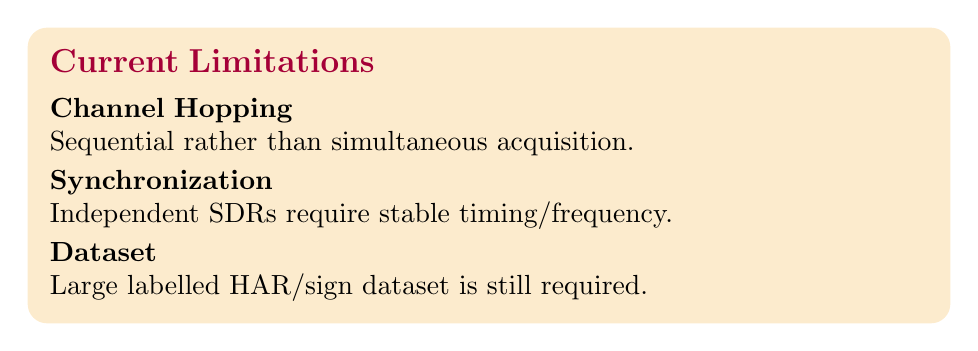
\begin{tikzpicture}
\node[
    rounded corners=7pt,
    fill=LightOrange,
    inner sep=8pt, % Reduced from 11pt
    text width=0.92\textwidth, % Increased slightly to reduce text wrapping
    align=left
] {
\textbf{\large\color{AmritaMaroon}Current Limitations}\\[4pt] % Reduced from 7pt

\textbf{Channel Hopping}\\
Sequential rather than simultaneous acquisition.\\[2pt] % Reduced from 5pt

\textbf{Synchronization}\\
Independent SDRs require stable timing/frequency.\\[2pt] % Reduced from 5pt

\textbf{Dataset}\\
Large labelled HAR/sign dataset is still required.
};
\end{tikzpicture}

\column{0.48\textwidth}

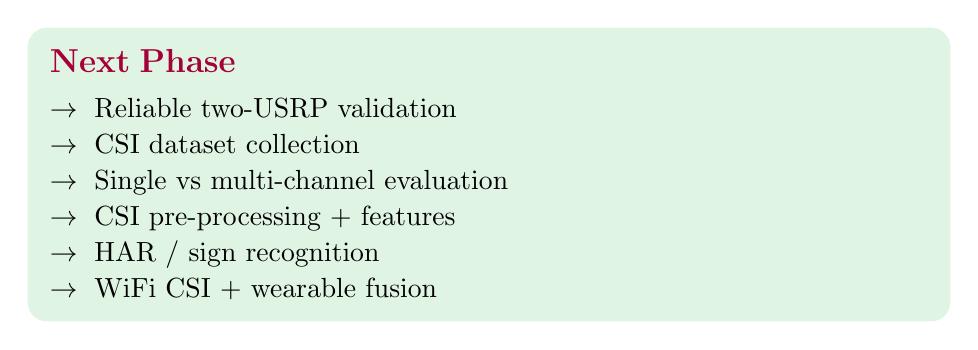
\begin{tikzpicture}
\node[
    rounded corners=7pt,
    fill=LightGreen,
    inner sep=8pt, % Reduced from 11pt
    text width=0.92\textwidth, % Increased slightly to reduce text wrapping
    align=left
] {
\textbf{\large\color{AmritaMaroon}Next Phase}\\[4pt] % Reduced from 7pt

$\rightarrow$\; Reliable two-USRP validation\\[1pt] % Reduced from 3pt
$\rightarrow$\; CSI dataset collection\\[1pt]
$\rightarrow$\; Single vs multi-channel evaluation\\[1pt]
$\rightarrow$\; CSI pre-processing + features\\[1pt]
$\rightarrow$\; HAR / sign recognition\\[1pt]
$\rightarrow$\; WiFi CSI + wearable fusion
};
\end{tikzpicture}

\end{columns}

\vspace{0.15cm} % Reduced from 0.35cm

\begin{center}
\textbf{\color{AmritaMaroon}Long-term goal:}
Sign-language recognition with identity-aware multi-modal sensing.
\end{center}

\end{frame}
% =========================================================
% 14. REFERENCES
% =========================================================

\begin{frame}{14. References}

\footnotesize % Changed from \small to prevent vertical overflow

\begin{columns}[T,totalwidth=\textwidth]

\column{0.48\textwidth}

\begin{enumerate}
\setlength{\itemsep}{3pt} % Tightened spacing between items

\item D. J. Cook et al.,
\textit{CASAS: A Smart Home in a Box},
Computer, 2013.

\item H. Alemdar et al.,
\textit{ARAS human activity datasets in multiple homes},
PervasiveHealth, 2013.

\item D. Anguita et al.,
\textit{A Public Domain Dataset for Human Activity Recognition},
ESANN, 2013.

\item R. Chavarriaga et al.,
\textit{The Opportunity challenge},
Pattern Recognition Letters, 2013.

\item D. Micucci et al.,
\textit{UniMiB SHAR},
Applied Sciences, 2017.

\item Y. Zheng et al.,
\textit{Widar3.0: Zero-Effort Cross-Domain Gesture Recognition},
IEEE TPAMI, 2021.

\end{enumerate}

\column{0.48\textwidth}

\begin{enumerate}
\setcounter{enumi}{6}
\setlength{\itemsep}{3pt} % Tightened spacing between items

\item G. Zhu et al.,
\textit{CSI-Bench},
arXiv, 2025.

\item S. Huang et al.,
\textit{WiMANS},
arXiv, 2024.

\item Y. Ma et al.,
\textit{SignFi: Sign Language Recognition Using WiFi},
ACM IMWUT, 2018.

\item J. Li et al.,
\textit{WiFinger: Finger Gesture Recognition Using CSI},
UbiComp, 2016.

\item B. D. Minor et al.,
\textit{Learning Activity Predictors from Sensor Data},
IEEE TKDE, 2017.

\vspace{0.15cm} % Reduced vertical space

\textbf{\color{AmritaMaroon}Implementation basis}\\
GNU Radio, UHD, IEEE 802.11 PHY/MAC processing,
and custom CSI extraction.

\end{enumerate}

\end{columns}

\end{frame}
% =========================================================
% THANK YOU
% =========================================================

\begin{frame}

\begin{center}

\vspace{1.2cm}

{\Huge\color{AmritaMaroon}\bfseries Thank You}

\vspace{0.5cm}

{\Large
Smart Home HAR for\\
Speech-Impaired \& Hearing-Impaired Users
}

\vspace{0.6cm}

\textbf{Guide Review 1 \;|\; Panel Review 1}

\vspace{0.4cm}

Department of Computer Science and Engineering\\
Amrita Vishwa Vidyapeetham

\end{center}

\end{frame}

\end{document}